\section{Gate Voltage and Charge Carrier Density}

To understand the influence of varrying densities of charge carriers $n$, the gate voltage $U_\text{gate}$ is varried. 
Gate voltages of  $1.5V, 1V, -0.25V, -1V, -1.5V$ were applied.
The first tree gate voltages are depicted in fig. \ref{fig:differentGateVoltagesQHE}.
They exhibit Hall plateaus and Shoubnikow-de Haas oscillations.
The Hall resistivity $\rho_\text{xy}$ grows slower with $B$ for larger densities of states.
Notice, that the plateaus in $\rho_\text{xy}$ remain at the same discrete values, but require higher $B$.
This can be explained with the higher Fermi level, which has more Landau niveaus with lower energy.
A higher $B$ is required to shift the Landau niveaus above the Fermi level.
\begin{figure}[h]
    \centering
    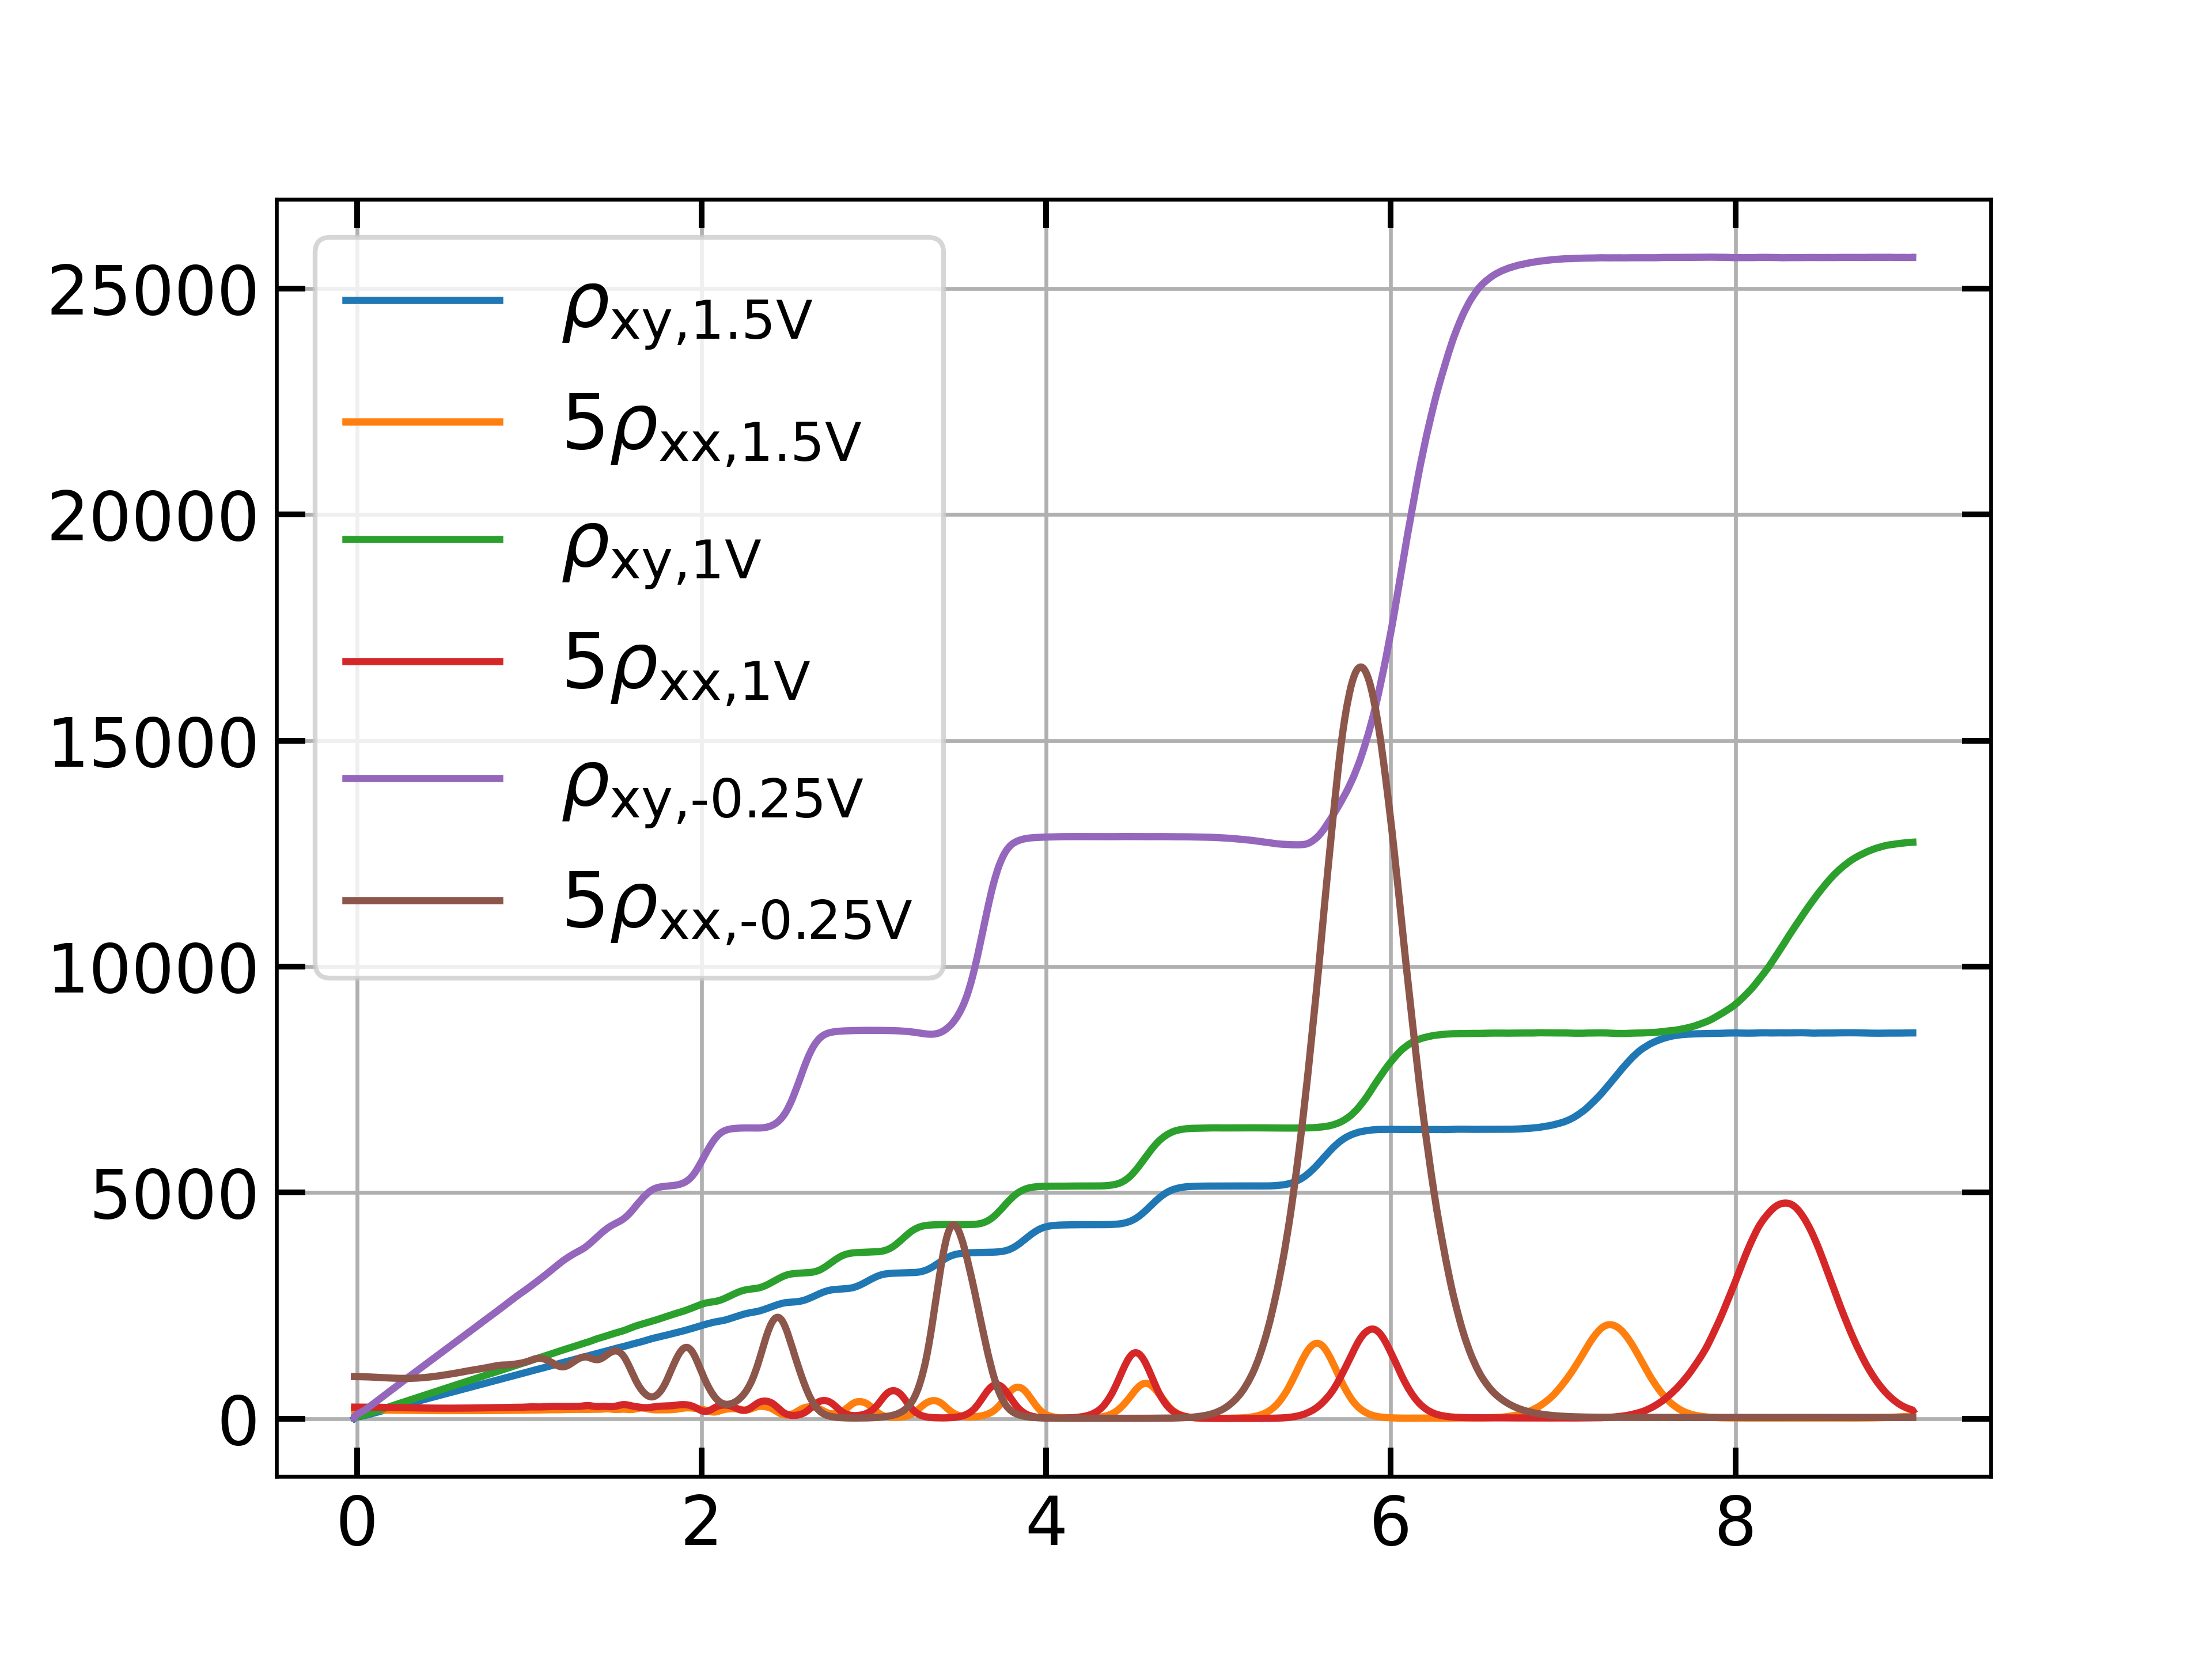
\includegraphics[width=0.45\textwidth]{../Images/differentGateVoltagesQHE.png}
    \caption{??}
    \label{fig:differentGateVoltagesQHE}
\end{figure}
In this tree cases, the fermi level remains above (or at, for $\nu=1$) the lowest Landau level.
Notice, that for fixed $n$ the lowest Landau niveau will not cross the Fermi level by increasing $B$.
The Fermi niveau can, however be shifted below the lowest landau level, if $U_\text{gate}$ and the corresponding $n$ is low enough.
Then only niveaus corresponding to defects are located around the Fermi level.
When lowering $U_\text{gate}$ even further, the Fermi level will cross the band gap from the conduction band to the valence band.
Further Landau niveaus should appear, but the corresponding charge carriers are no longer electrons, but holes.
This effect is investigated with $U_\text{gate}=-1V,\,-1.5V$.
The resistivities for these gate voltages are plotted in \ref{fig:kaputteKurvenGateV}.
\begin{figure}[h]
    \centering
    
\includegraphics[width=0.45\textwidth]{../Images/kaputteKurvenGateV.png}
    \caption{??}
    \label{fig:kaputteKurvenGateV}
\end{figure}
For the gate voltage of $1V$, the charge carrier density is very small, resulting in the steep incline of $\rho_\text{xy}$.
This explains, why the plateau corresponding to $\nu=1$ is already reached for $B\approx1.6T$ and 
the plateaus corresponding to  $\nu\>1$ are not visible.
The longitudinal component has vanishing resistivity for the values of $B$, for which \rhall has the plateau.  
After further increasing $B$, \rhall temporarily shows negative values.
This could be explained by p-type conduction, since the holes with positive charges, 
moving in the other direction are deflected in the same direction as electrons, resulting in a change of sign in \rhall.





Since the valence band typically has a lower curvature near the band gap, the holes typically have a larger effective mass $m^\star$.
The cyclotron frequency
\begin{align}
    \omega_c = \frac{eB}{m^\star}    
\end{align}
an therefore the energy (difference) of the Laudau levels
\begin{align}
    \varepsilon = \hbar \omega_c \left(\frac{1}{2} + n_\textL \right)    
\end{align}
is smaller.
This makes the Landau levels harder to seperate. 
Larger $B$ would be required to accieve the same results as with electrons.








Extrapolating $n$ for lower $U_\text{gate}$ gives an estimate for the charge carrier density (see fig. \ref{})
\begin{figure}[h]
    \centering
    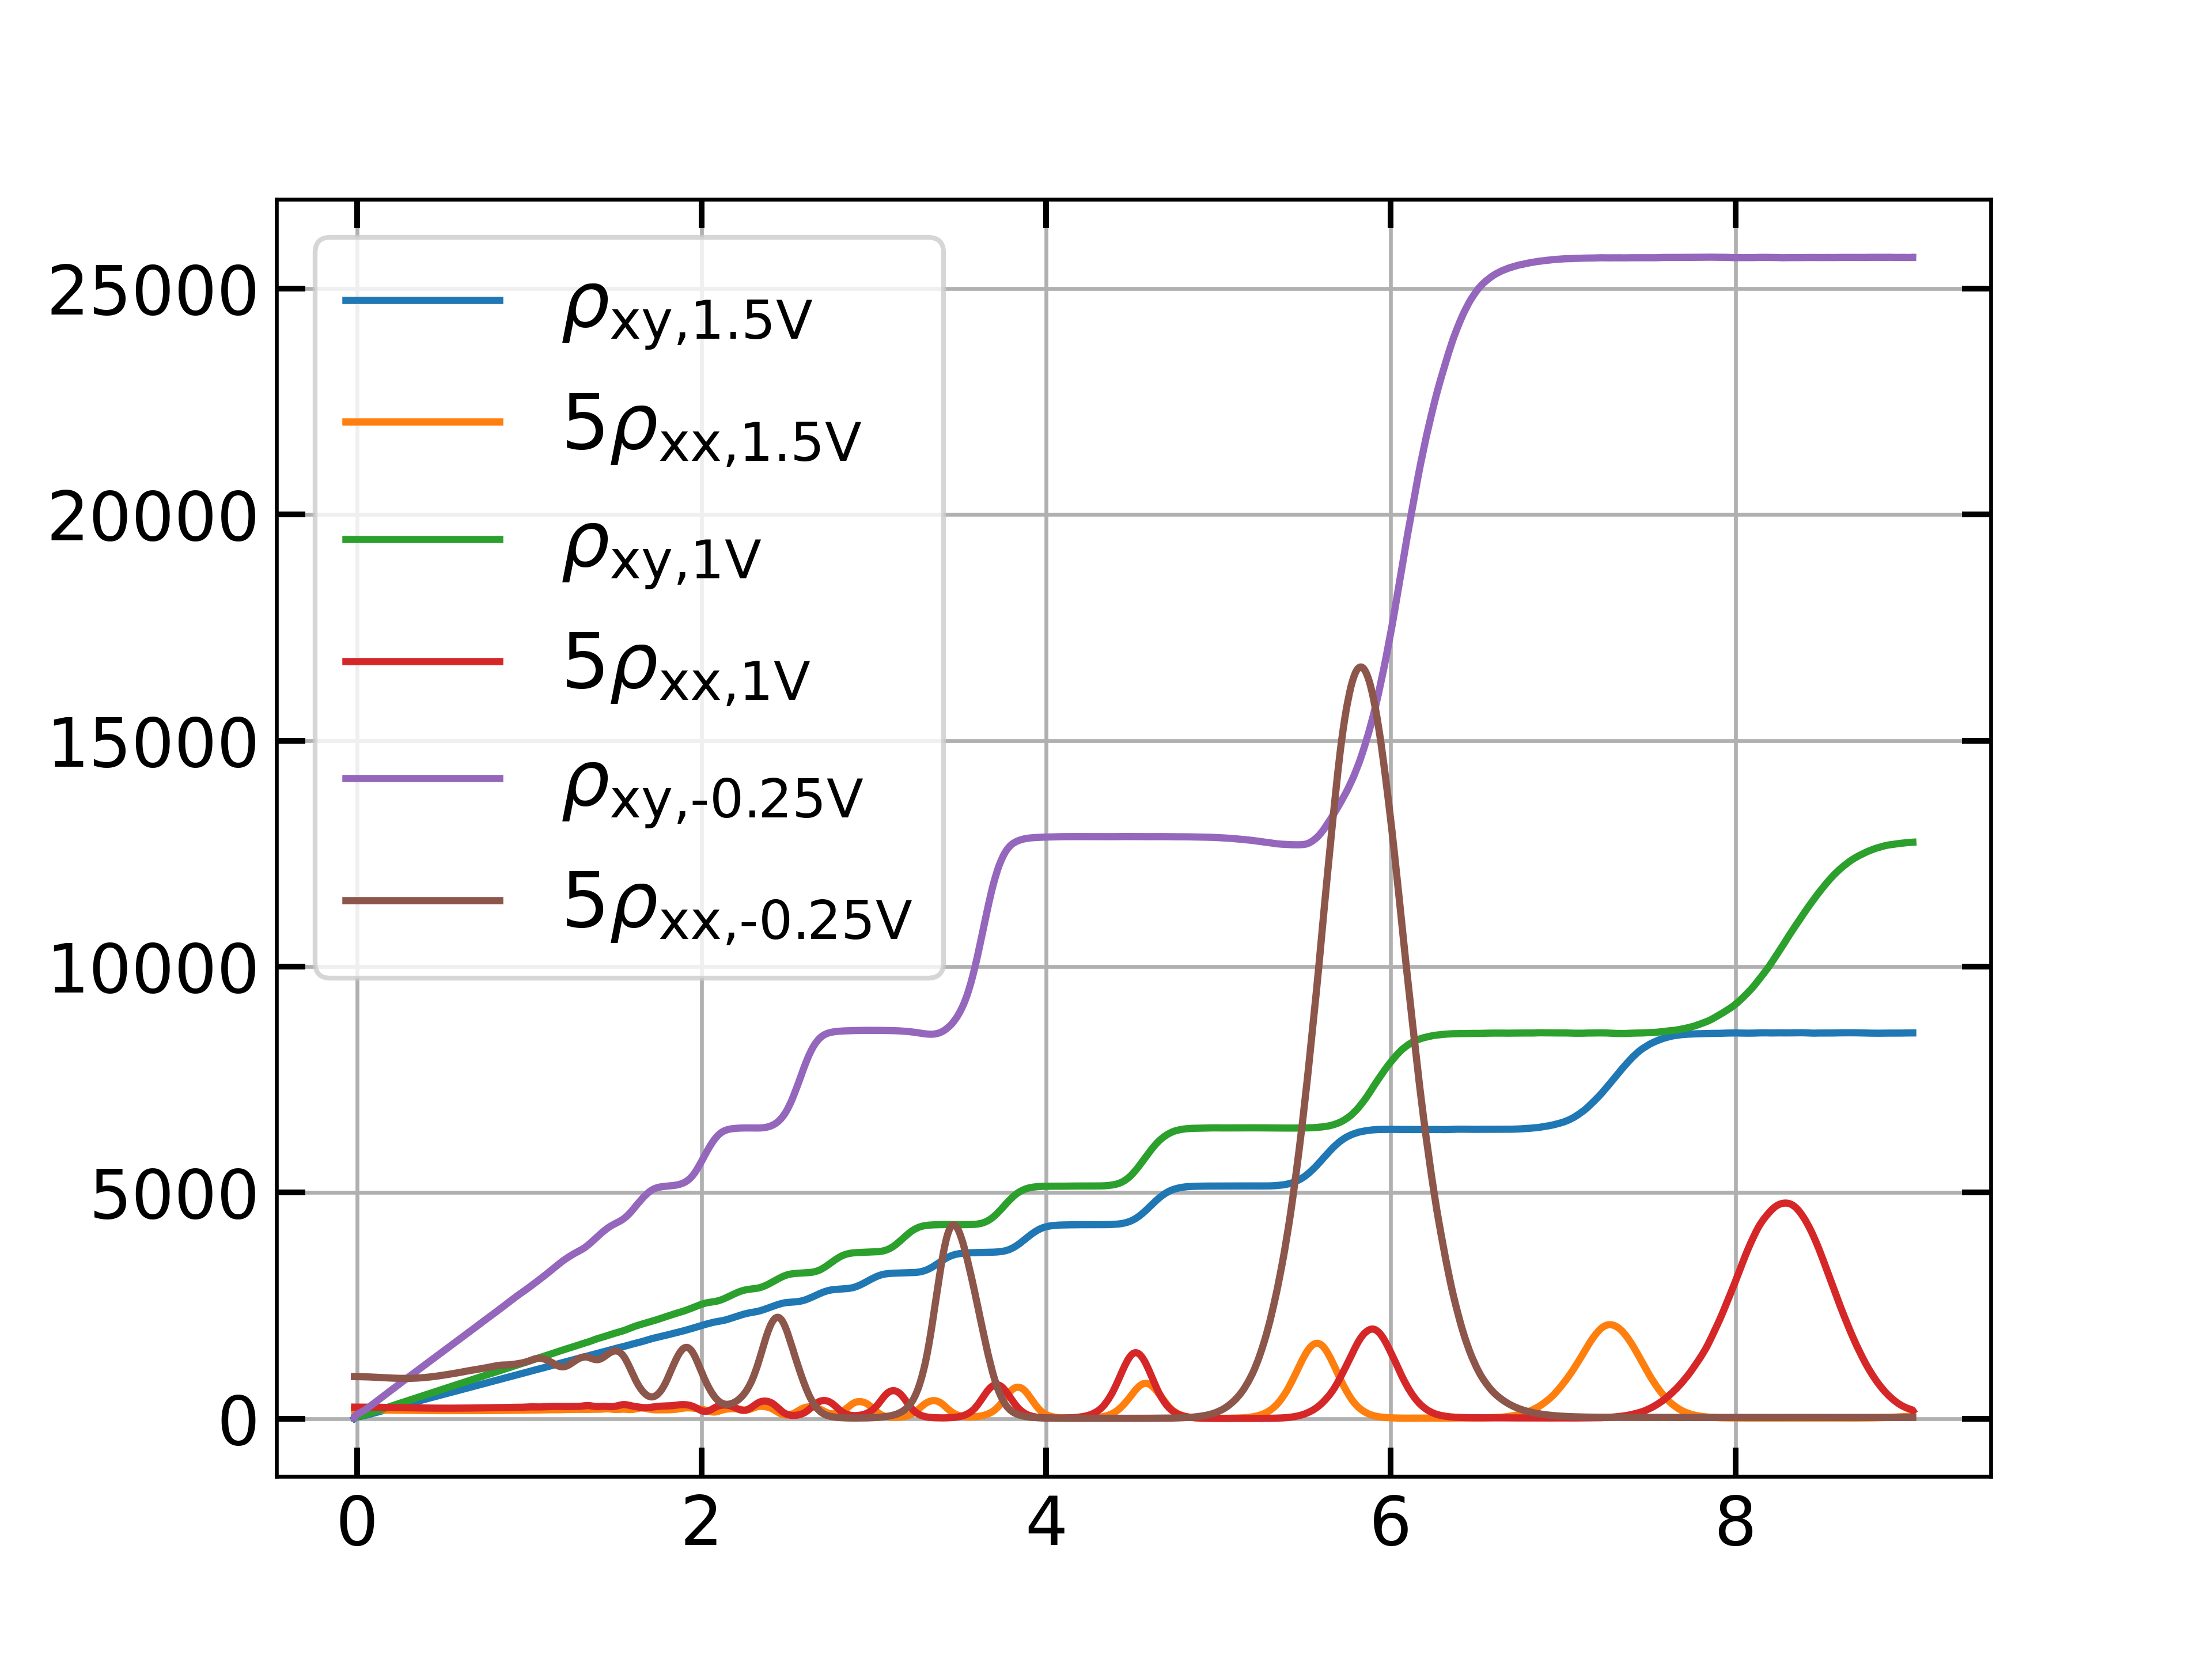
\includegraphics[width=0.45\textwidth]{../Images/differentGateVoltagesQHE.png}
    \caption{??}
    \label{fig:differentGateVoltagesQHE}
\end{figure}




However, this behaviour is expected     


